%%
%% TO BUILD A PDF FILE: uncomment the following line, comment the SVG line below, and run "pdflatex flowchart.tex"
%%
\documentclass[crop,tikz]{standalone}

%%
%% TO BUILD A SVG FILE: comment the PDF line above, uncomment the line following line, and run "pdflatex -shell-escape flowchart.tex"
%%
%\documentclass[crop,tikz,convert={outfile=\jobname.svg}]{standalone}

\pagestyle{empty}
\usepackage[utf8]{inputenc}
\usepackage{tikz}

\usetikzlibrary{shapes.geometric, arrows}

\tikzstyle{box} = [rectangle, rounded corners, minimum width=3cm, minimum height=1cm,text centered, draw=black, thick, fill=green!30]
\tikzstyle{redBox} = [rectangle, rounded corners, minimum width=3cm, minimum height=1cm,text centered, draw=black, thick, fill=red!30]
\tikzstyle{yellowBox} = [rectangle, rounded corners, minimum width=3cm, minimum height=1cm, text centered, draw=black, thick, fill=yellow!30]
\tikzstyle{yellowBoxRedBorder} = [rectangle, rounded corners, minimum width=3cm, minimum height=1cm, text centered, draw=red, thick, fill=yellow!30]
\tikzstyle{plainBox} = [rectangle, rounded corners, minimum width=3cm, minimum height=1cm, text centered, draw=black, thick]
\tikzstyle{plainBoxRedBorder} = [rectangle, rounded corners, minimum width=3cm, minimum height=1cm, text centered, draw=red,thick]

\tikzstyle{dataBox} = [rectangle, rounded corners, minimum width=9.0cm, minimum height=4.9cm,text centered, draw=black,thick, fill=gray!10]
\tikzstyle{invariantBox} = [rectangle, rounded corners, minimum width=5.5cm, minimum height=6.9cm,text centered, draw=black,thick, fill=blue!10]

\tikzstyle{arrow} = [thick,->,>=stealth]

\begin{document}
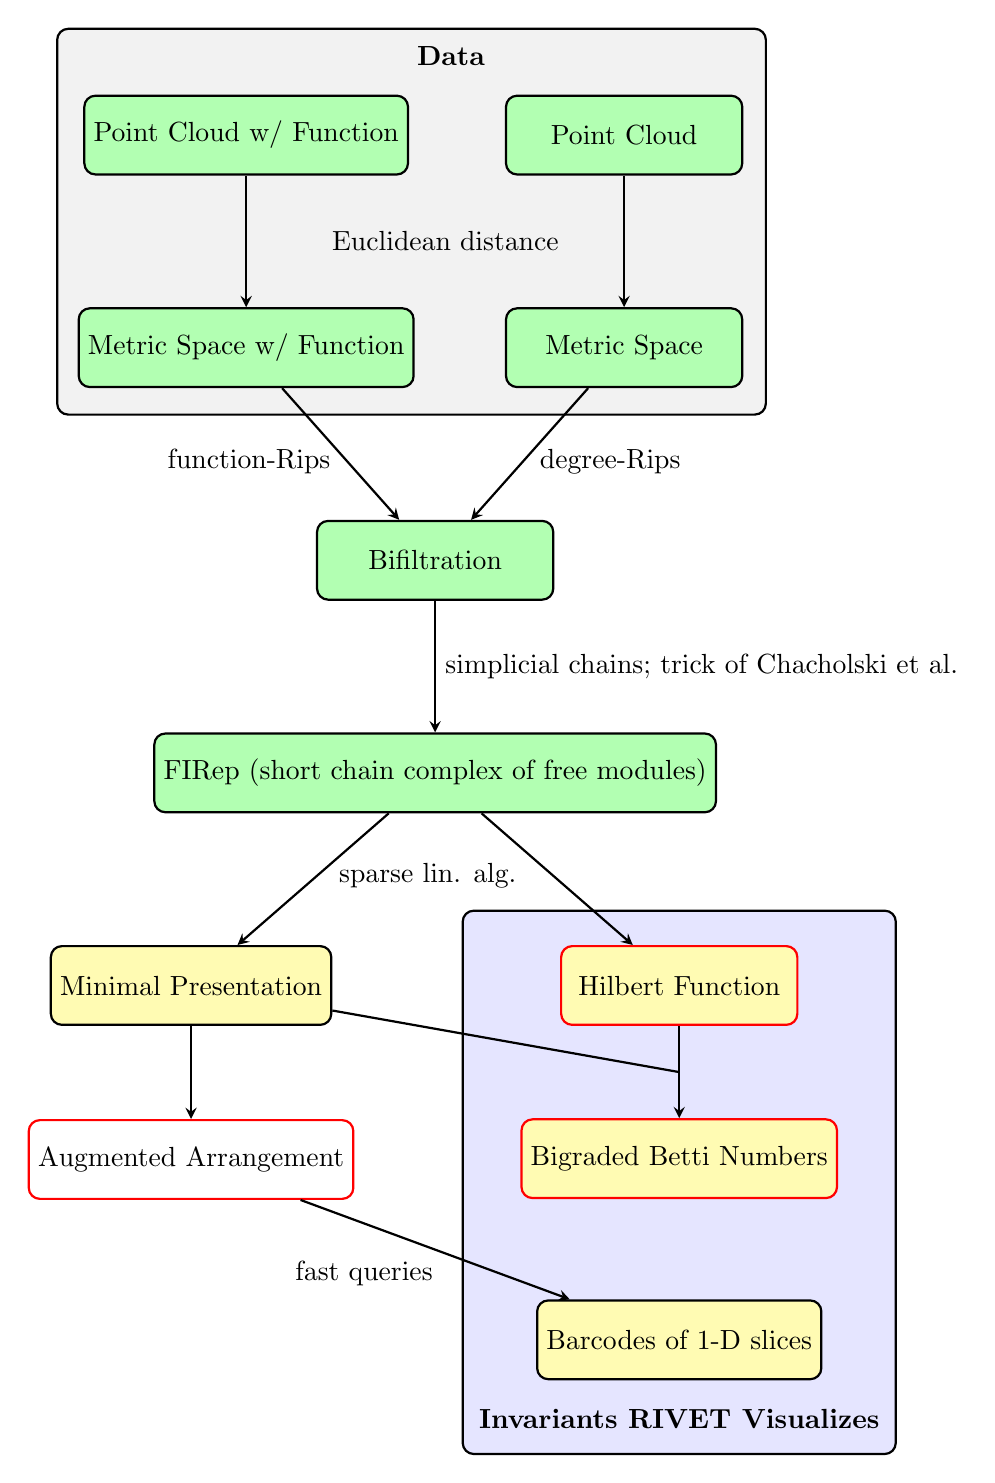
\begin{tikzpicture}[node distance=1.9cm]

\node (data) [dataBox,yshift=-2.1cm,xshift=-.3cm] {};
\node (dataLabel)[xshift=.2cm] {\textbf{Data}};

\node (pointsAnchor) [yshift = -1cm] {};
\node (metricAnchor) [below of= pointsAnchor] {};
\node (pointsFun) [box,left of=pointsAnchor,xshift=-.5cm] {Point Cloud w/ Function};
\node (points) [box,right of=pointsAnchor,xshift=.5cm] {Point Cloud};
\node (metricFun) [box,left of=metricAnchor,xshift=-.5cm,yshift=-.8cm] {Metric Space w/ Function};
\node (metric) [box,right of=metricAnchor,xshift=.5cm,yshift=-.8cm] {Metric Space};

\node (bifiltration) [box, below of=metricAnchor,yshift=-1.6cm] {Bifiltration};
%\node (input) [yellowBox,left of= bifiltration, xshift=-5cm] {Text File Input};

\node (firep) [box, below of=bifiltration,yshift=-.8cm] {FIRep (short chain complex of free modules)};

\node (magicAnchor) [below of= firep,yshift=-.8cm] {};
\node (minpres) [yellowBox, left of=magicAnchor,xshift=-1.2cm] {Minimal Presentation};

\node (invariant) [invariantBox,right of= magicAnchor,xshift=1.2cm,yshift=-2.5cm] {};
\node (invariantLabel) [below of=invariant,yshift=-1.1cm] {\textbf{Invariants RIVET Visualizes}};
\node (hilbert)[yellowBoxRedBorder, right of= magicAnchor,xshift=1.2cm]{Hilbert Function};

\node (bettiCombine) [coordinate,below of= hilbert,yshift=.8cm] {};
\node (betti) [yellowBoxRedBorder, below of= bettiCombine,yshift=.8cm]{Bigraded Betti Numbers};
\node (arrangement)[plainBoxRedBorder, below of= minpres,yshift=-.31cm] {Augmented Arrangement};
\node (barcodes)[yellowBox, below of= betti, yshift=-.4cm]  {Barcodes of 1-D slices};
%\node (visualization)[plainBox, below of= barcodes,yshift=-1cm]  {Visualization};
%\node (minpres) [box, below of=firep, yshift=-0.5cm] {Minimal Presentation};
%\node (pro2a) [process, below of=minpres, yshift=-0.5cm] {};
%\node (pro2b) [process, right of=minpres, xshift=2cm] {Process 2b};
%\node (out1) [io, below of=pro2a] {Output};
%\node (stop) [box, below of=out1] {Stop};
%\draw [arrow] (input) -- (data);
%\draw [arrow] (input) -- (bifiltration);
%\draw [arrow] (input) -- (firep);
\draw [arrow] (points) --  node[anchor=east,xshift=-0.7cm]{Euclidean distance} (metric);
\draw [arrow] (pointsFun) --  (metricFun);
\draw [arrow] (metric) -- node[anchor=west,yshift=-.1cm]{degree-Rips}(bifiltration);
\draw [arrow] (metricFun) -- node[anchor=east,yshift=-.1cm]{function-Rips} (bifiltration);
\draw [arrow] (bifiltration) -- node[anchor=west]{simplicial chains; trick of Chacholski et al.} (firep);
\draw [arrow] (firep) -- node[anchor=west,xshift=.2cm,yshift=.05cm]{sparse lin. alg.} (minpres);
\draw [arrow] (firep) -- (hilbert);
\draw [thick] (minpres) -- (bettiCombine);
\draw [thick] (hilbert) -- (bettiCombine);
\draw [arrow] (bettiCombine) -- (betti);
%\draw [thick] (betti) -- node[anchor=west,xshift=-1.7cm,yshift=.4cm]{line arrangement}(arrangementCombine);
\draw [arrow] (minpres) -- (arrangement);
%\draw [arrow] (invariant) -- (visualization);
%\draw [arrow] (minpres) -- node[anchor=east] {yes} (pro2a);
%\draw [arrow] (minpres) -- node[anchor=south] {no} (pro2b);
%\draw [arrow] (pro2b) |- (firep);
%\draw [arrow] (pro2a) -- (out1);
%\draw [arrow] (out1) -- (stop);

\draw [arrow] (arrangement) -- node[anchor=east,xshift=.1cm,yshift=-.3cm]{fast queries} (barcodes);
\end{tikzpicture}

\end{document}